\subsection{ZKPK of representation}

Proof knowledge of $\alpha_i$ such that $y = \prod g_i^{\alpha_i}$:

\[
		PK\{ (\alpha_1, \alpha_2, \ldots, \alpha_n) : y = g_1^{\alpha_1} \cdot \ldots \cdot g_n^{\alpha_n} \}
\]

Where the DL base $g_i$ of $g_j$ is unknown for all $i \neq j$.

\begin{algorithm}
		\caption{ZKPK of representation}

		\begin{multicols}{2}
				\begin{algorithmic}[0]
						\State \textbf{A}
						\State $r_i \rgets \mathbb{Z}_q$
						\State $t \coloneqq \prod g_i^{r_i} \rightarrow$
						\State
						\State $s_i \coloneqq r_i - c \cdot \alpha_i \rightarrow$
				\end{algorithmic}

				\columnbreak

				\begin{algorithmic}[0]
						\State \textbf{B}
						\State
						\State
						\State $\leftarrow c \rgets \mathbb{Z}_q$
						\State \textbf{Verify} $t = (\prod g_i^{s_i}) \cdot y^c$
				\end{algorithmic}
		\end{multicols}
\end{algorithm}

Applicability: Prove knowledge of plaintext $m$ of additively homomorphic
ElGamal ciphertext $(R, C) = (g^r, g^m \cdot y^r)$: $C = g^m \cdot y^r$.

\subsection{Proof of equality}

Proof that $DL_{g_1}(y_1) = DL_{g_2}(y_2)$:

\[
		PK\{ (\alpha) : y_1 = g_1^\alpha \land y_2 = g_2^\alpha \}
\]

\begin{algorithm}
		\caption{ZKPK of equality}

		\begin{multicols}{2}
				\begin{algorithmic}[0]
						\State \textbf{A}
						\State $r \rgets \mathbb{Z}_q$
						\State $t_i \coloneqq g_i^r \rightarrow$
						\State
						\State $s \coloneqq r - c \cdot x \rightarrow$
				\end{algorithmic}

				\columnbreak

				\begin{algorithmic}[0]
						\State \textbf{B}
						\State
						\State
						\State $\leftarrow c \rgets \mathbb{Z}_q$
						\State
						\State \textbf{Verify} $t_i = g_i^s \cdot y_i^c$
				\end{algorithmic}
		\end{multicols}
\end{algorithm}

Applicability: Prove that additively homomorphic ElGamal ciphertext $(R, C) =
(g^r, g^m \cdot y^r)$ is a valid encryption of $m \in \{0, 1\}$ by combining
with proof of disjunction: $\log_g(R) = \log_y(C / g^0) \lor \log_g(R) = \log_y(C / g^1)$

\subsection{Proof of conjunction (AND)}

Idea: Use same challenge in two parallel proofs.

\subsection{Proof of disjunction (OR)}

Assume $P$ only knows $x_b$, not $x_{b'}$. Wants to prove $PK\{ (x_1, x_2)
: \Phi_1(y_1, x_1) \lor \Phi_2(y_2, x_2) \}$.

\begin{algorithm}
		\caption{ZKPK of disjunction}

		\begin{multicols}{2}
				\begin{algorithmic}[0]
						\State \textbf{A}
						\State $(t_b, r_b) \coloneqq \operatorname{commit}(y_b)$
						\State Fake proof for $x_{b'}$
						\State $c_{b'} \coloneqq \operatorname{challenge}()$
						\State $(t_{b'}, r_{b'}, s_{b'}) \coloneqq \operatorname{simulate}(y_{b'}, c_{b'})$
						\State $\xrightarrow{t_0, t_1}$
						\State
						\State $c_b \coloneqq c + c_{b'}$
						\State $s_b \coloneqq \operatorname{response}(x_b, y_b, t_b, r_b, c_b)$
						\State $\xrightarrow{c_0, s_0, c_1, s_1}$
				\end{algorithmic}

				\columnbreak

				\begin{algorithmic}[0]
						\State \textbf{B}
						\State
						\State
						\State
						\State
						\State
						\State $\leftarrow c \coloneqq \operatorname{challenge}()$
						\State
						\State
						\State \textbf{Verify} $c_0 + c_1 = c \land \operatorname{verify}(y_1, y_1, c_1, s_1) \land \operatorname{verify}(y_2, t_2, c_2, s_2)$
				\end{algorithmic}
		\end{multicols}
\end{algorithm}

\subsection{Making ZKPK non-interactive}

Remove interactino by computing challenge $c$ using a one-way function from
$t$. Called `Fiat-Shamir transformation'.

Example from Schnorr proof:
\begin{enumerate}
		\item $c \coloneqq H(t || m)$. In this case $m$ added as some context
				of message $m$.
		\item Output simulated transcript $(t, s)$ of ZKPK
\end{enumerate}

\subsection{Discrete-log based commitments}

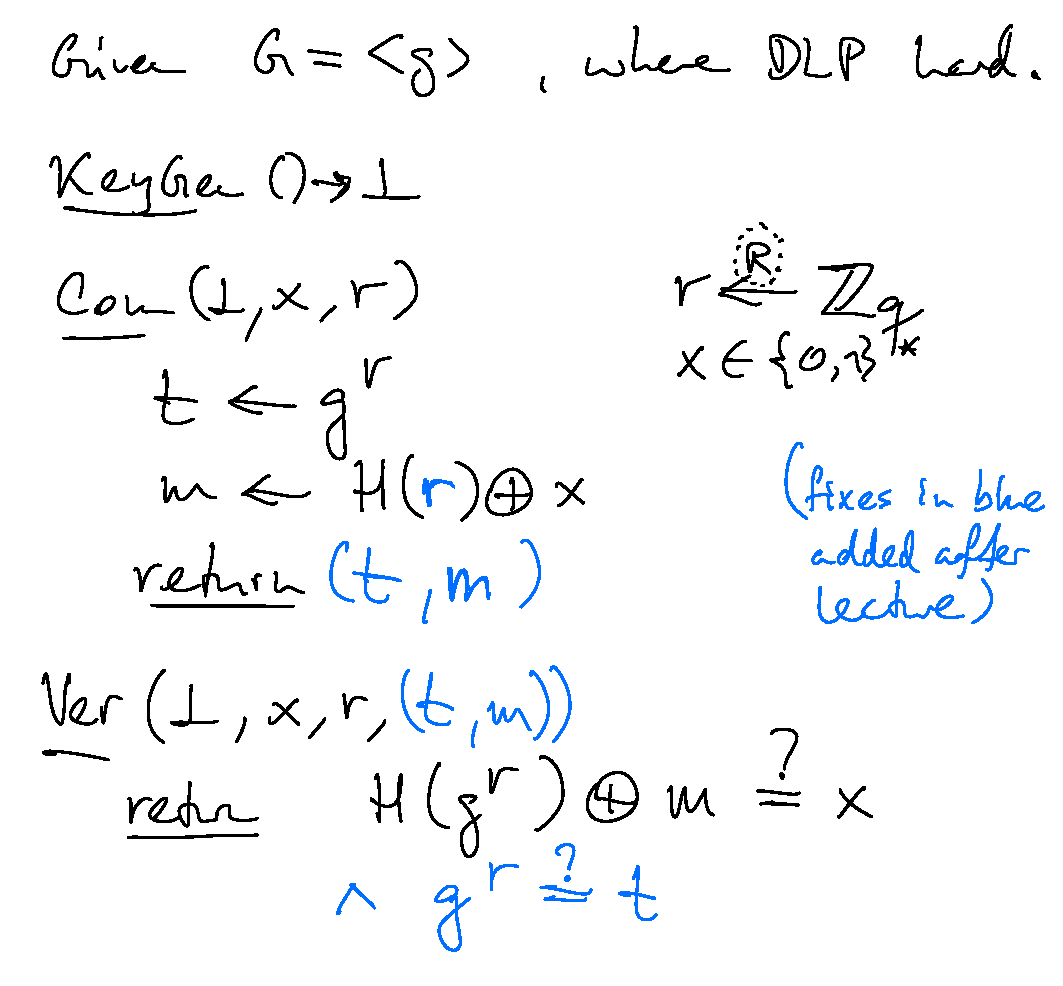
\includegraphics[width=\textwidth]{06_dl_commitments}

\subsection{Pedersen commitments}

Given $G = <g> = <h>$, $g, h$ generated independently (e.g. trusted setup).


\begin{algorithm}
		\caption{Pedersen-based commitment scheme}

		\begin{algorithmic}[0]
				\Procedure{KeyGen}{}
						\State $h \rgets G$
						\State \textbf{Return} $h$
				\EndProcedure

				\Procedure{Commit}{$h, x, r$}
						\State $r \rgets \mathbb{Z}_q$
						\State \textbf{Return} $g^x \cdot h^r$
				\EndProcedure

				\Procedure{Verify}(h, x, r, c)
						\State \textbf{Return} $c == g^x \cdot h^r$
				\EndProcedure
		\end{algorithmic}
\end{algorithm}

Information-theoretically unconditionally hiding. But need to convince all
parties that generators were computed correctly (i.e. independently).
